\documentclass{article}
\usepackage{tikz}
\begin{document}
\begin{center}
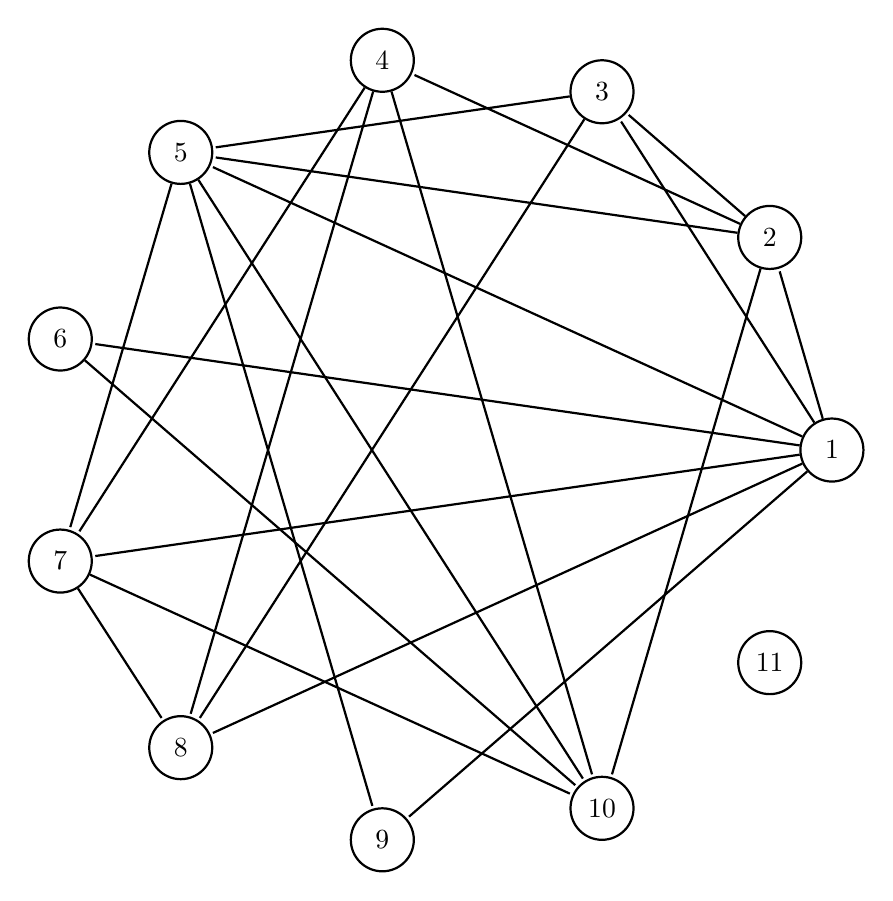
\begin{tikzpicture}[>=stealth,shorten >=1pt,auto,node distance=3cm,thick]
\tikzstyle{every node}=[circle,draw,minimum size=8mm]

\node (1) at (5.00,0.00) {1};
\node (2) at (4.21,2.70) {2};
\node (3) at (2.08,4.55) {3};
\node (4) at (-0.71,4.95) {4};
\node (5) at (-3.27,3.78) {5};
\node (6) at (-4.80,1.41) {6};
\node (7) at (-4.80,-1.41) {7};
\node (8) at (-3.27,-3.78) {8};
\node (9) at (-0.71,-4.95) {9};
\node (10) at (2.08,-4.55) {10};
\node (11) at (4.21,-2.70) {11};

\draw (5) -- (7);
\draw (5) -- (10);
\draw (1) -- (6);
\draw (2) -- (5);
\draw (1) -- (3);
\draw (1) -- (9);
\draw (7) -- (10);
\draw (4) -- (8);
\draw (5) -- (9);
\draw (2) -- (4);
\draw (1) -- (2);
\draw (1) -- (5);
\draw (2) -- (10);
\draw (1) -- (8);
\draw (6) -- (10);
\draw (4) -- (7);
\draw (3) -- (5);
\draw (4) -- (10);
\draw (3) -- (8);
\draw (2) -- (3);
\draw (1) -- (7);
\draw (7) -- (8);
\end{tikzpicture}
\end{center}
\end{document}
